\documentclass[12pt]{article}

\usepackage{amsmath}
\usepackage{vntex}
\usepackage{titling}
\usepackage{graphicx}
\usepackage[table,xcdraw]{xcolor}
\usepackage{float}

\title{
    \textbf{Automatic plant watering system}\\
}
\author{
    \textit{Author:}\\
    Phạm Đức Anh Khoa - 2053140\\
    Nguyễn Thị Ngọc Nhi - 2052632\\
    Mai Minh Nhật - 2053295\\
    Nguyễn Tôn Minh - 2052600 \\~\\
    \textit{A report for Electrical - Electrical circuit subject}\\
    \textit{Faculty of}\\
    \textit{Computer Science and Engineering}
    }
\date{
    
\includegraphics[scale = 0.6]{./images/Logo_BK.png}\\~\\
    \textbf{Viet Nam National University Ho Chi Minh} \\
    Ho Chi Minh University of Technology
    }

\begin{document}
    \maketitle
    \thispagestyle{empty}

    \newpage

    \section{Design}
    \subsection{Power consumption of the circuit}
    The following components' power consumption values are provided by the seller.\\
    \begin{table}[H]
    \centering
    \begin{tabular}{|l|c|}
         \hline
         \textbf{Components} & \textbf{Power Consumption} \\ \hline
         Humidity sensor & 0.025W \\ \hline
         OLED 0.91-inch I2C & 0.03W \\ \hline
         5V water pump & 0.66W \\ \hline
         Red LED & 0.01W \\ \hline
         Green LED & 0.01W \\ \hline
         Arduino Uno & 5.0W \\ \hline
         Relay Module (5V - 10A) & 0.05W \\ \hline
         Joystick & 0.05W \\ \hline
         \textbf{Total} & \textbf{5.835W} \\ \hline
    \end{tabular}
    \end{table}

    After checking out most electronic shops, we came to the conclusion of using a 12V - 450mA power supply, which can supply 5.4W of power, for the circuit we intended to build. Even though the power supplied by the source is less than the total power consumption of the circuit, a deficiency of 0.435W did not affect the performance of our circuit after thorough testing so we decided to keep it.
    \newpage
    \subsection{How components work}
        \subsubsection{OLED screen}
            OLED screen is basically a matrix with RGB LEDs, the library on Arduino IDE helps user render each pixel as an LED.
            \begin{figure}[!h]
                \centering
                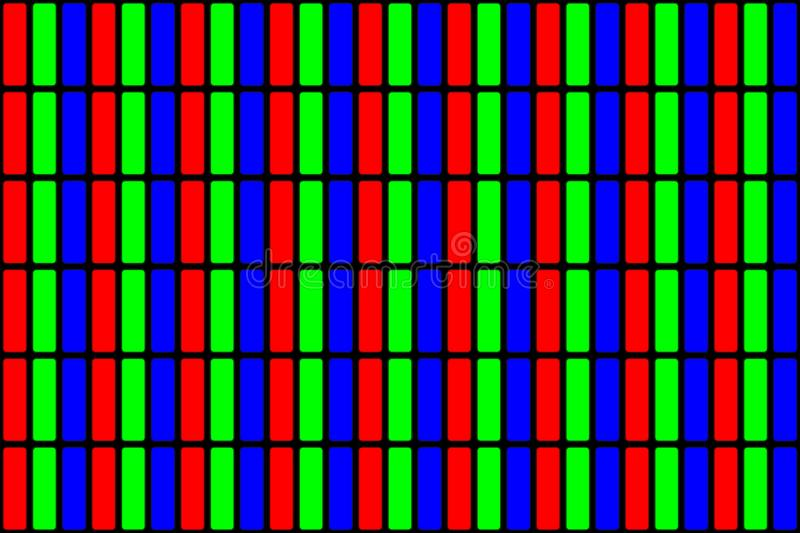
\includegraphics[scale = 1]{./images/OLED.jpg}
                \caption{OLED screen zoom in}
                \label{fig:OLED}
            \end{figure}

        \subsubsection{Arduino Uno}
            \begin{itemize}
                \item Example of an Arduino UNO:
                \begin{center}
                    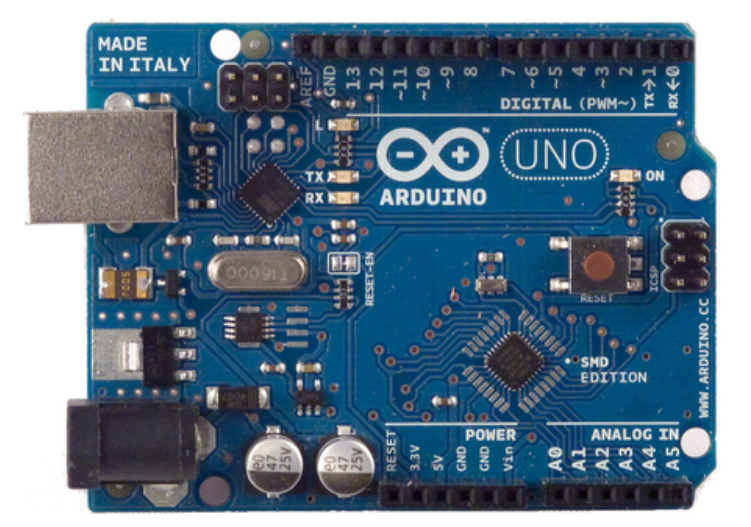
\includegraphics[scale = 0.6]{./images/arduino uno.png}     
                \end{center}
                \item \textbf{Arduino Uno} is a programmable microcontroller that can plug in external devices and sensors.
                \item It can be programmed using \textbf{Arduino IDE}.
                \begin{center}
                    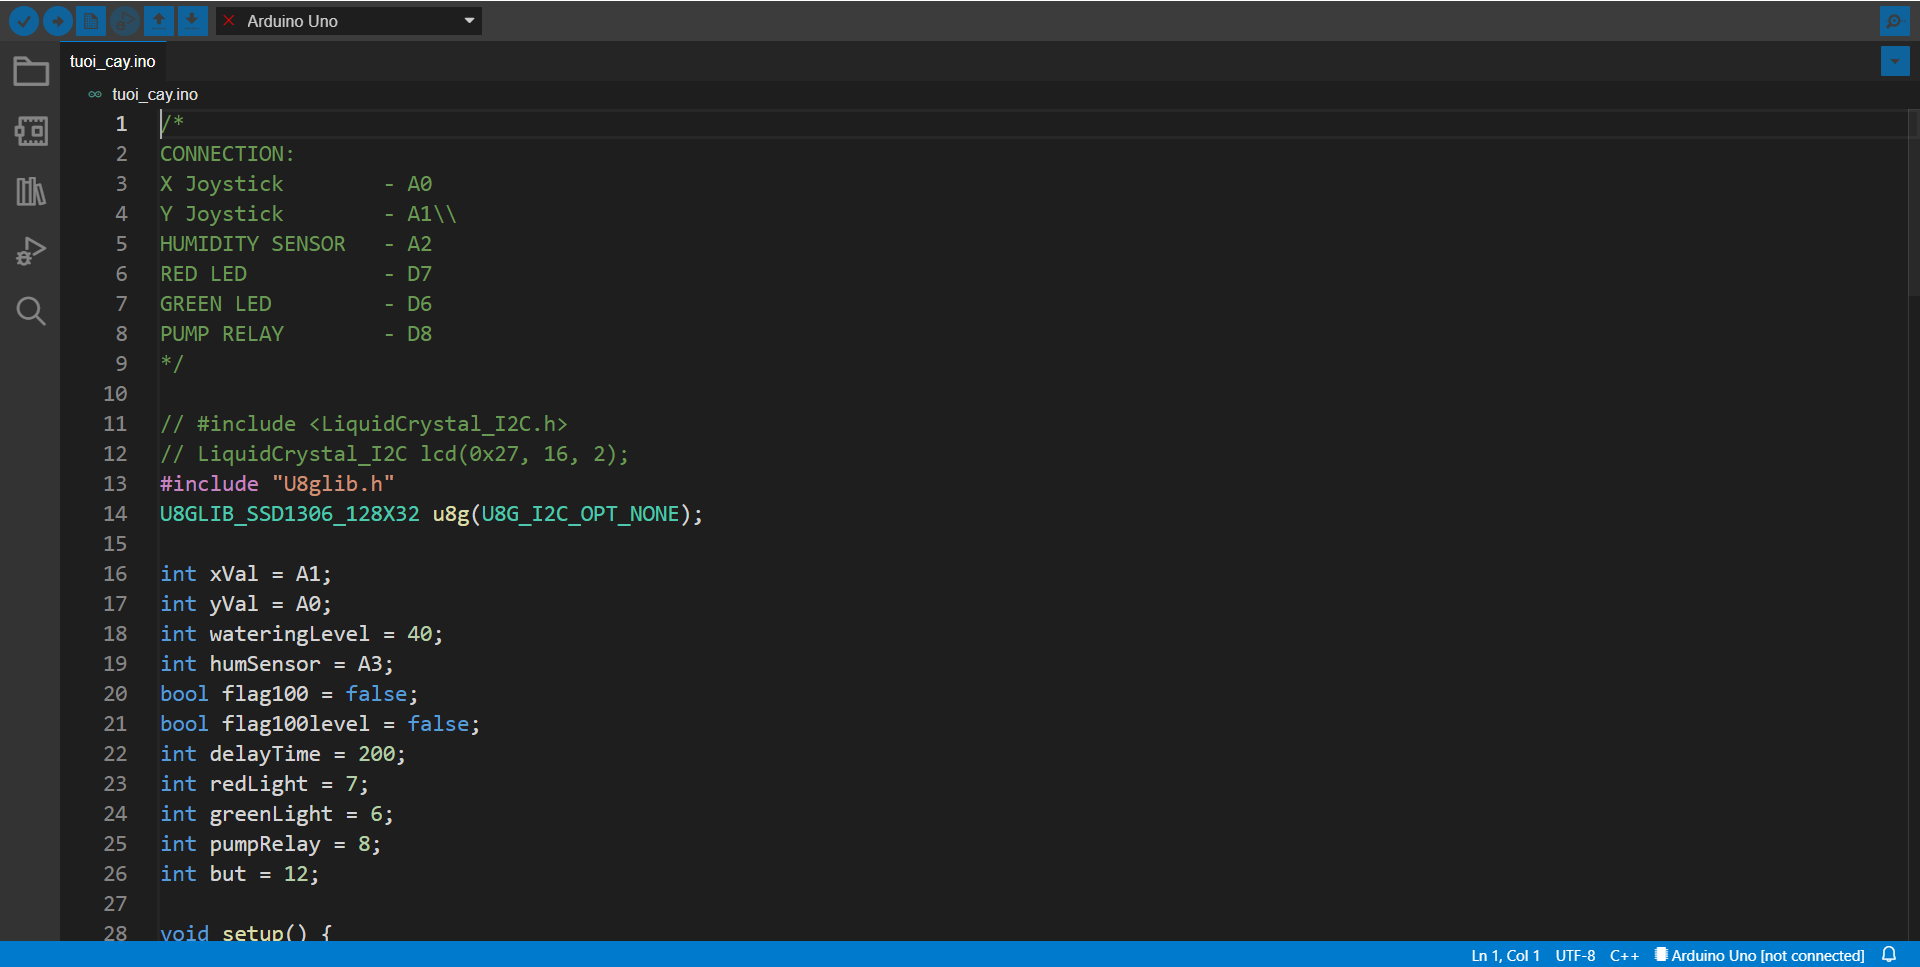
\includegraphics[scale = 0.3]{./images/arduino ide.png}    
                \end{center}
            \end{itemize}

        \subsubsection{Relay}
            \begin{itemize}
                \item Example of a relay:
                \begin{center}
                    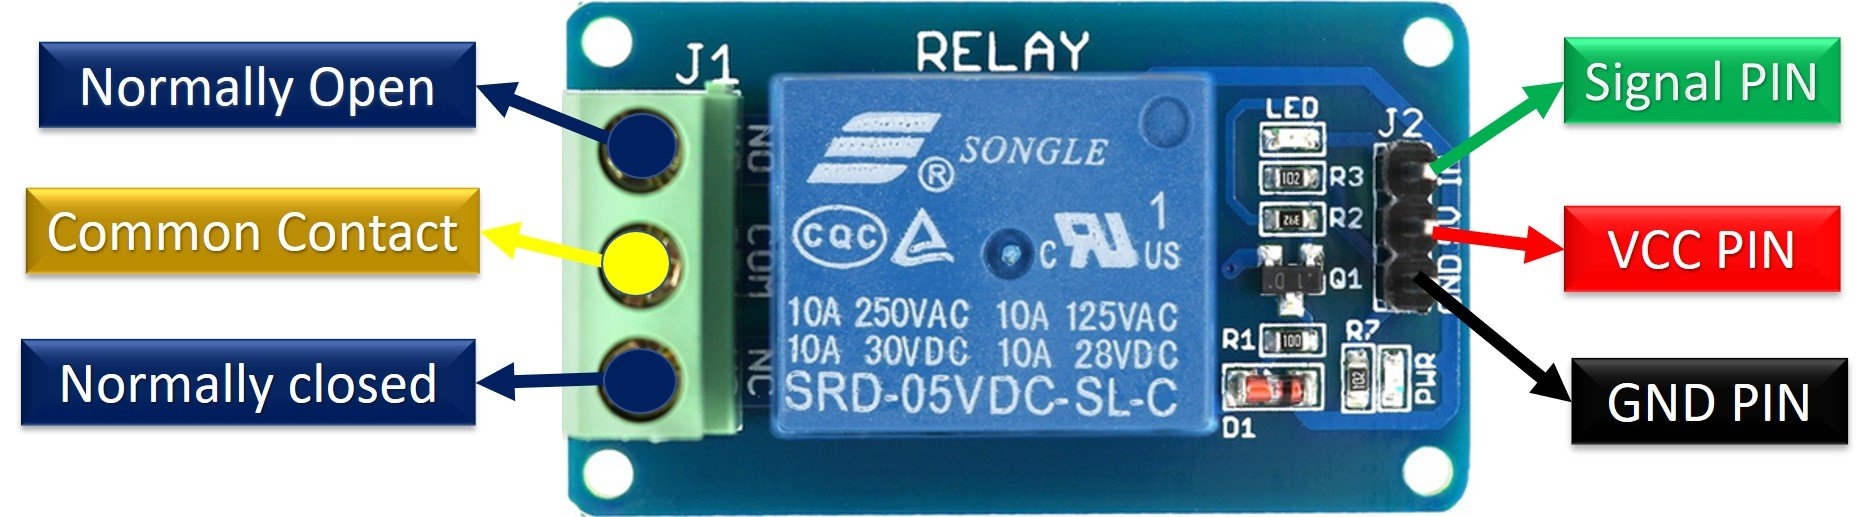
\includegraphics[scale = 0.2]{./images/relay.jpg}
                \end{center}

                \item Relay schematic: 
                \begin{figure}[!h]
                    \centering
                    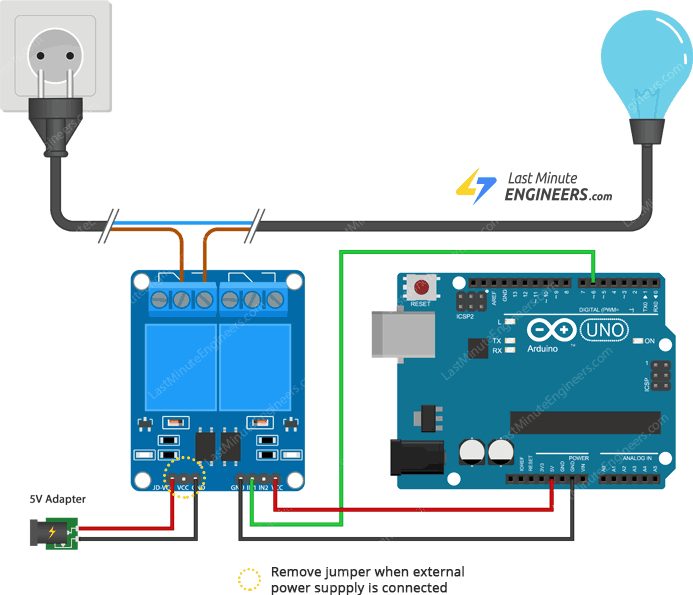
\includegraphics[scale = 3]{./images/relay_schematic.png}
                    \caption{Relay schematic}
                    \label{fig:relay schematic}
                \end{figure}

                \item Functionality: Whenever the \textbf{Signal pin} receive a \textbf{high signal}, the magnet will connect the \textbf{NO and COM}. We will use this function of the relay to activate the water pump.
            \end{itemize}

        \subsubsection{Joystick}
            \begin{itemize}
                \item Example of a joystick:
                \begin{center}
                    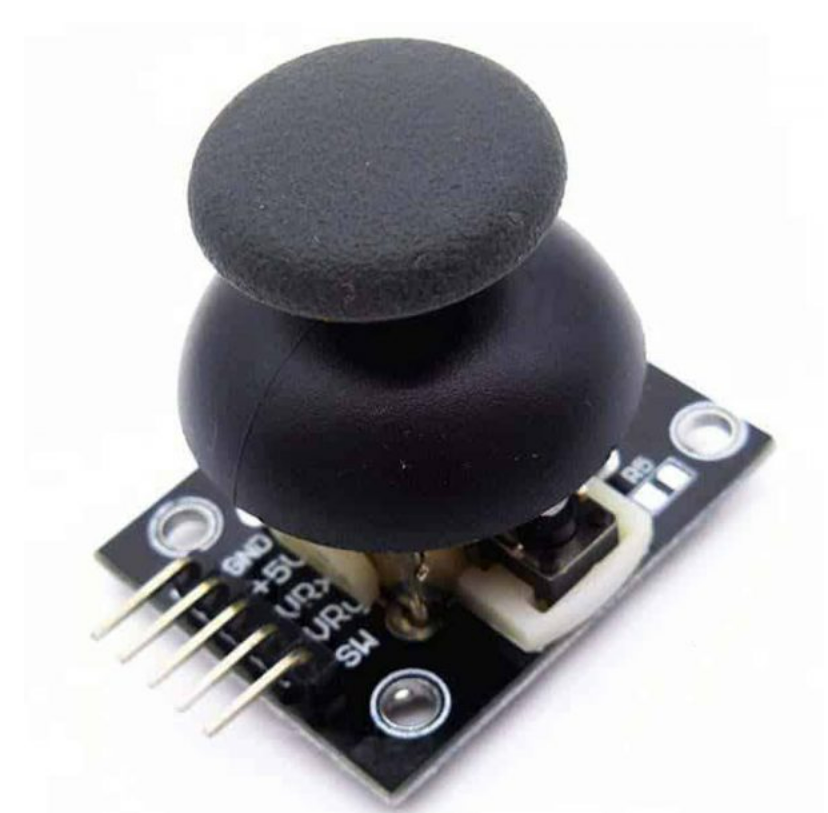
\includegraphics[scale = 0.25]{./images/joystick.png}
                \end{center}

                \item Joystick schematic:
                \begin{center}
                    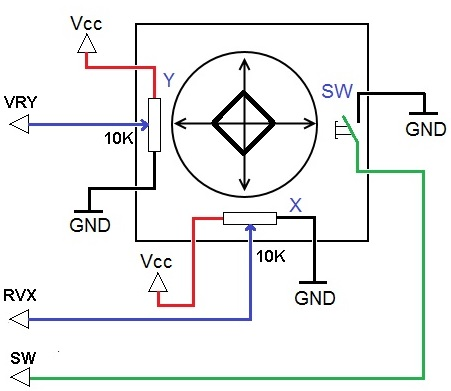
\includegraphics[scale = 0.75]{./images/joystick_schematic.jpg}
                \end{center}

                \item Functionality: The \textbf{VRx and VRy} is each attached to $10$k variable resistor, when user move the josytick, the variable resistor will change the value of output voltage and can be read by analog pin of Arduino UNO which goes from 0 to 1023.
            \end{itemize}

        \subsubsection{Full wave rectifier}
            \begin{itemize}
                \item Example of a 12V-450mA full wave rectifier:
                \begin{center}
                    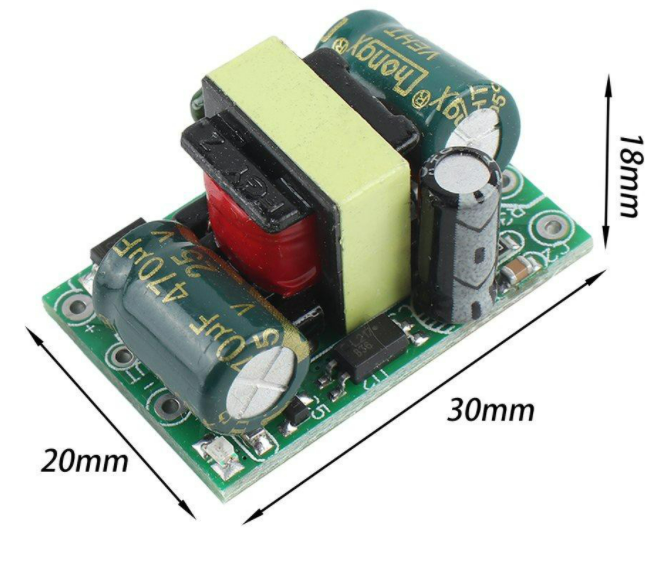
\includegraphics[scale = 0.5]{./images/ac-dc.png}
                \end{center}

                \item Functionality: turn 220V-50Hz AC power supply to 12V-450mA DC power supply
                % \item Schematic:
                % \begin{center}
                %     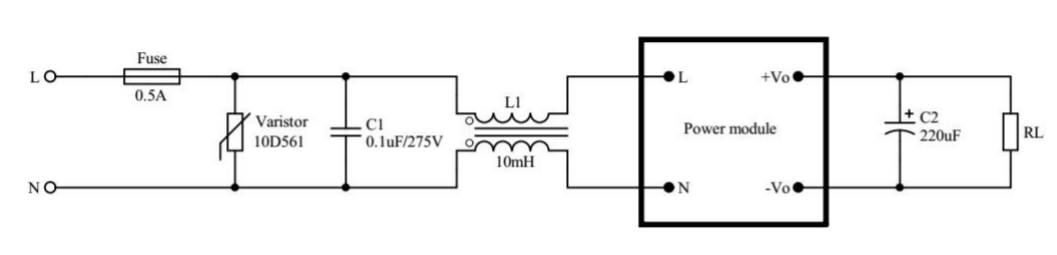
\includegraphics[scale = 0.6]{./images/ac-dc schematic.png}
                % \end{center}
            \end{itemize}

        \subsubsection{Capacitive humidity sensor}
            \begin{itemize}
                \item Example of a Capacitive humidity sensor:
                \begin{center}
                    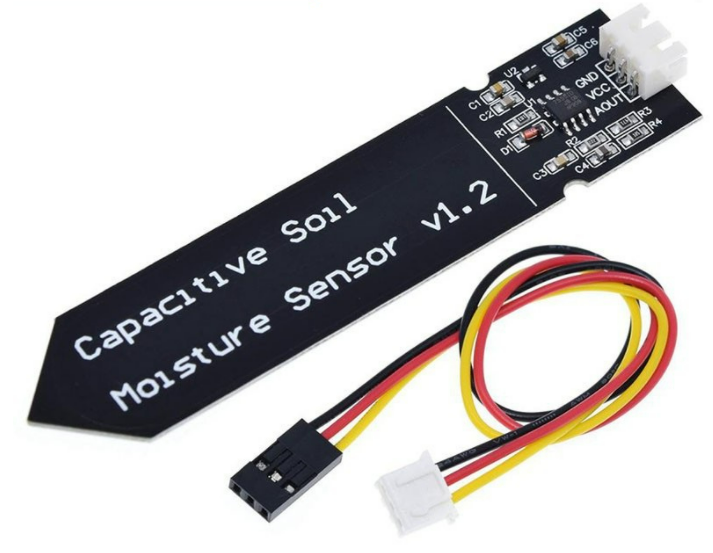
\includegraphics[scale = 0.5]{./images/hum_sensor.png}
                \end{center}

                \item Functionality: Determine humidity of dirt.
            \end{itemize}

        \subsubsection{T89 power supply}
            \begin{itemize}
                \item Example of a T89 power supply:
                \begin{center}
                    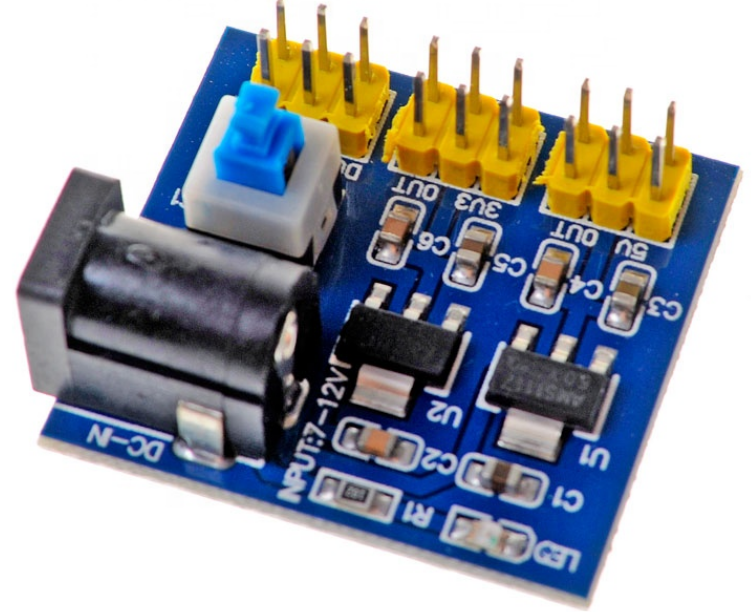
\includegraphics[scale = 0.25]{./images/t89.png}
                \end{center}

                \item Functionality: Using 2 DC voltage regulator to convert input voltage into 5V and 3.3V.
            \end{itemize}
    \newpage
    \subsection{Schematic of the circuit}
    After choosing the power supply, we did a mock schematic of the circuit with all the suitable parts we could find on the market.
    \begin{figure}[H]
        \centering
        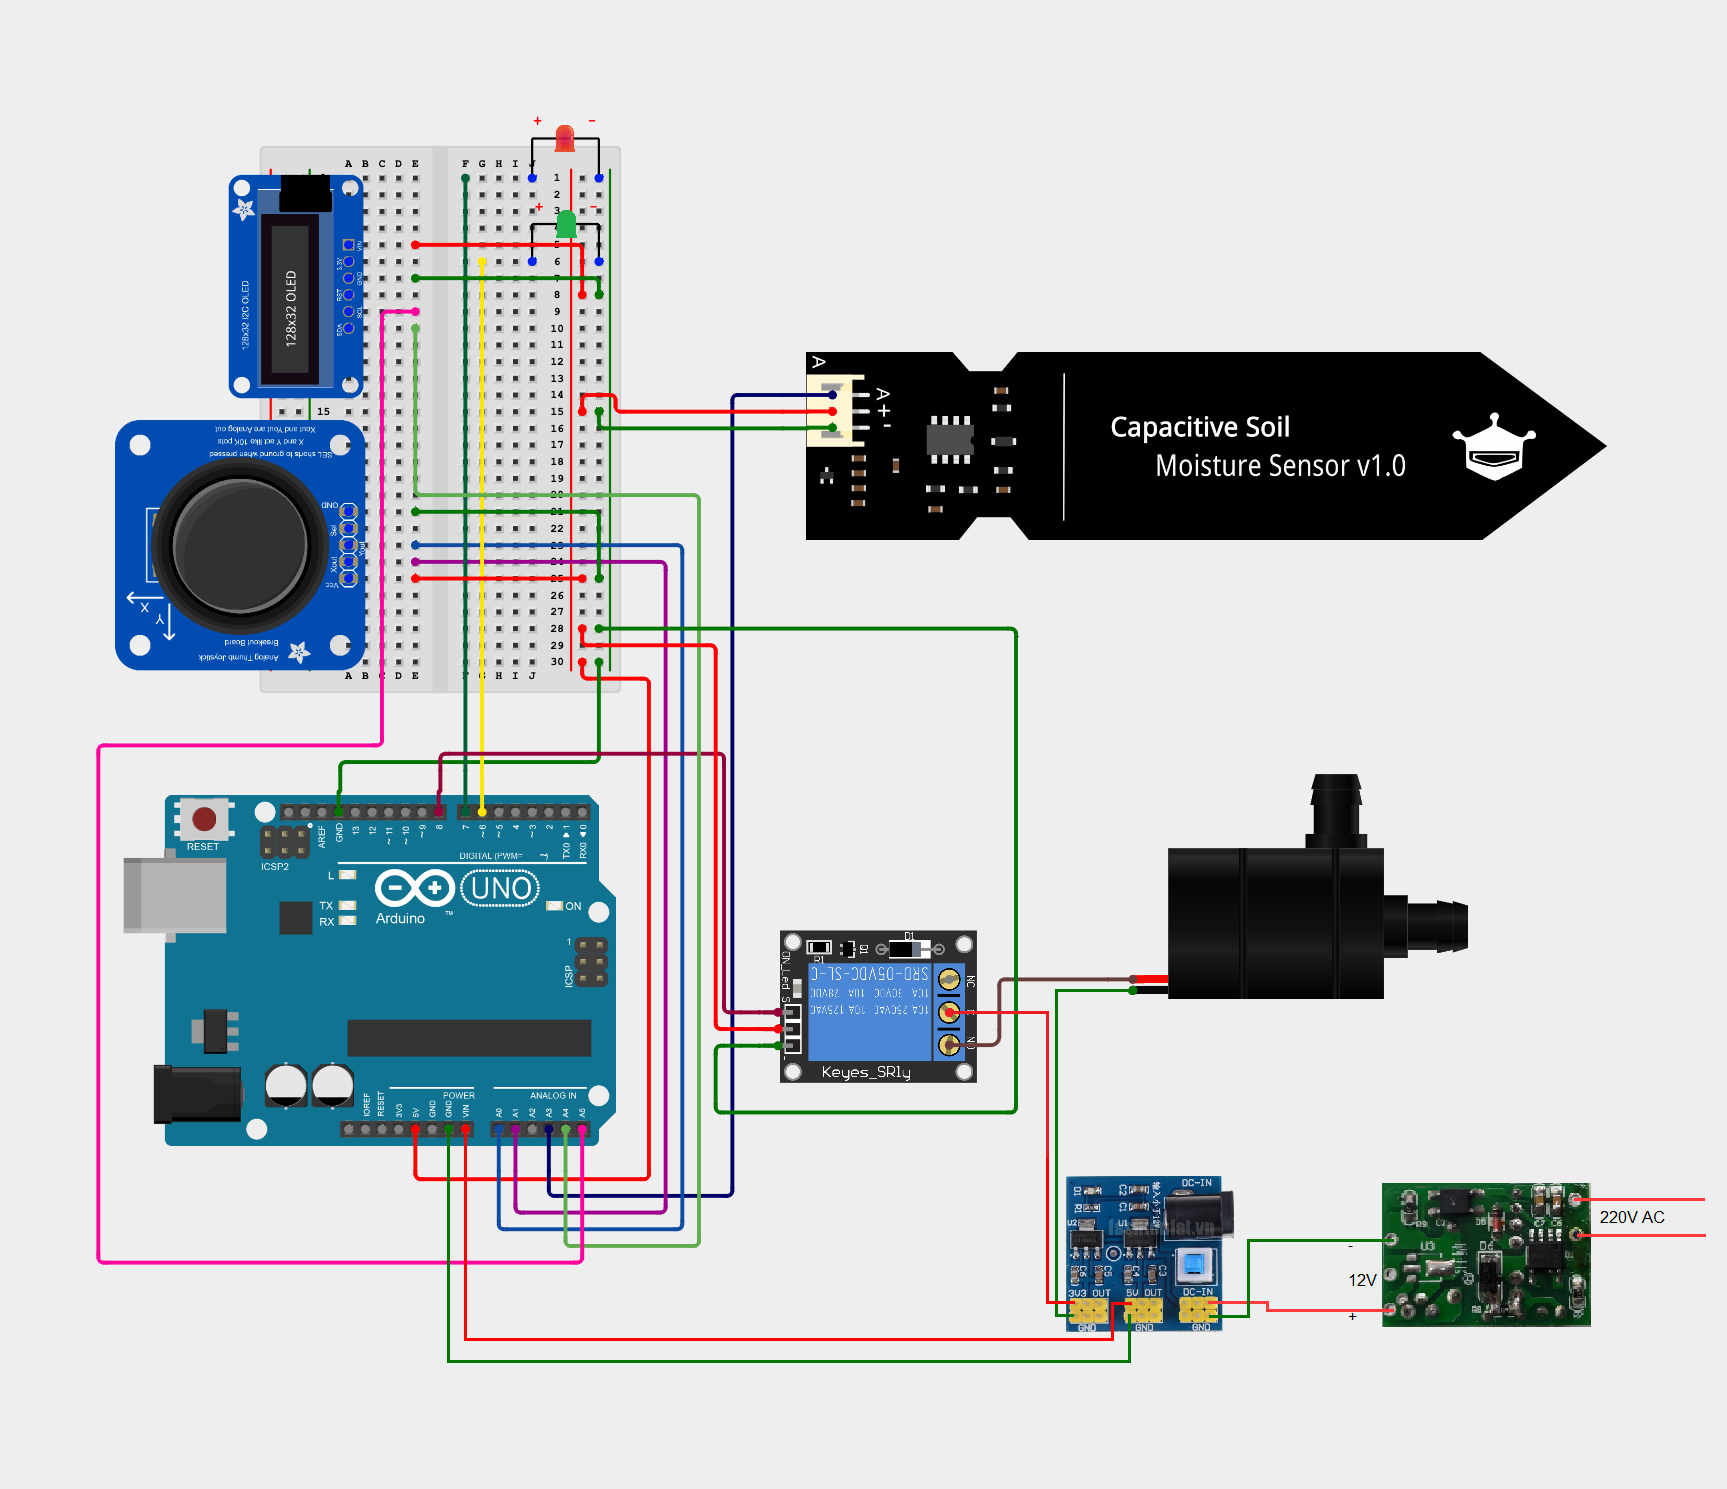
\includegraphics[width=14cm]{./images/breadboard.png}
        \caption{Schematic of the automatic plant watering system}
        \label{fig:schematic}
    \end{figure}
    \subsection{Pipeline}
    \begin{center}
        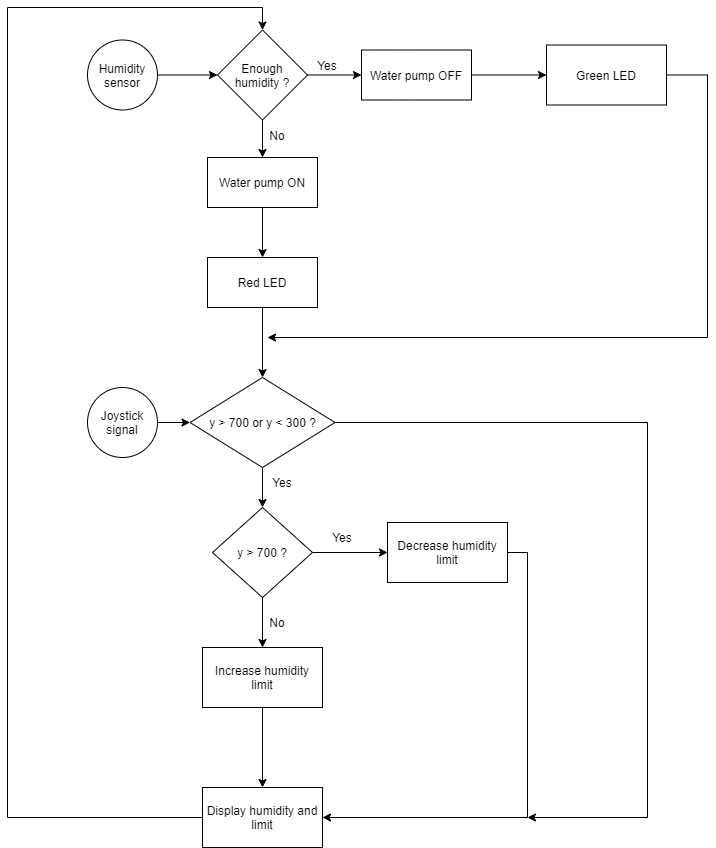
\includegraphics[scale = 0.5]{./images/flow chart.png}
    \end{center}
    \newpage
    \subsection{Arduino code}
    \begin{figure}[H]
        \centering
        
\includegraphics[width=14cm]{./images/include_lib.png}
        \caption{Include the OLED display library}
        \label{fig:include_lib}
    \end{figure}
    
    First, we include the OLED display on line 13 and let the library know we are using I2C connection on line 14.
    
    \begin{figure}[H]
        \centering
        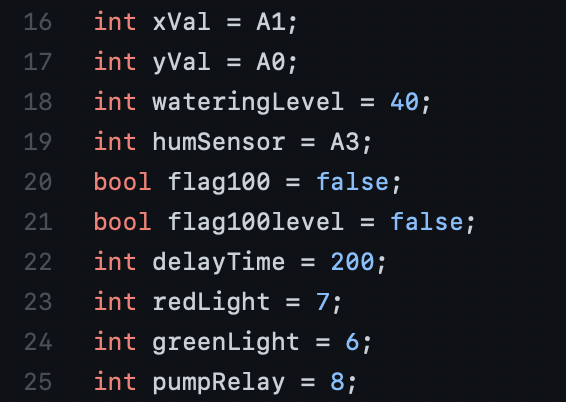
\includegraphics[width=14cm]{./images/assign.png}
        \caption{Declare variables and assign analog/digital connection or integer value to them}
        \label{fig:my_label}
    \end{figure}
    
    Here, we assign the x-axis and y-axis of the joystick to A1 and A0 respectively. We set the moisture level indicating that plants need watering to 40 (on a scale from 0 to 100). The humidity sensor is connected to A3. We set the delay time to 200 milliseconds and assign green LED, red LED and the relay module to digital port 6, 7 and 8 respectively.
    
    \begin{figure}[H]
        \centering
        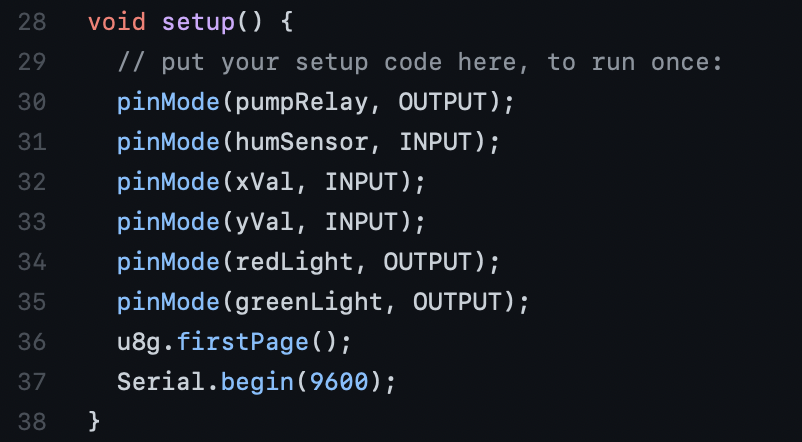
\includegraphics[width=14cm]{./images/setup.png}
        \caption{Setting up inputs and outputs}
        \label{fig:steup}
    \end{figure}
    
    Then we setup the components as inputs or outputs of the circuit.
    
    \begin{figure}[H]
        \centering
        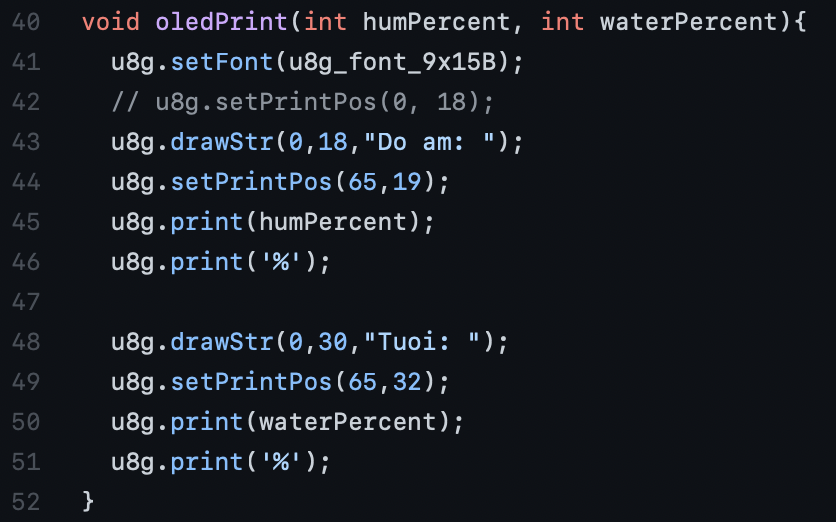
\includegraphics{./images/OLED_print.png}
        \caption{Function for printing on the OLED display}
        \label{fig:OLED_print}
    \end{figure}
    
    We print "Do am: " at coordinate (0, 18) and integer humPercent with '\%' at coordinate (65, 19). Similarly, we print "Tuoi: " at coordinate (0, 30) and integer waterPercent with '\%' at coordinate (65, 32).
    
    \begin{figure}[H]
        \centering
        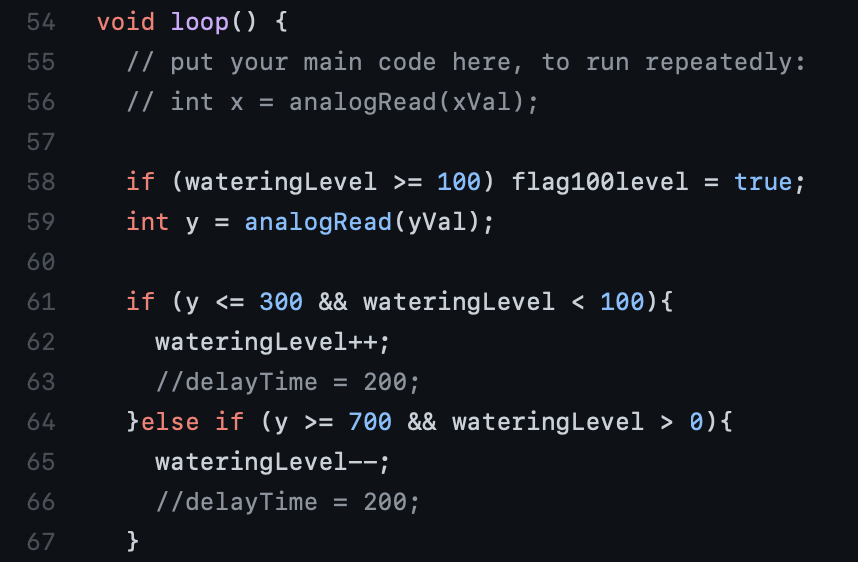
\includegraphics[width=14cm]{./images/main1.png}
        \caption{First part of the main code}
        \label{fig:main1}
    \end{figure}
    
    We declare an integer y and assign it with the value of the y-axis of the joystick. Then we make an if-else-if statement that increases the watering level when we move the y-axis of the joystick within the range from 0 to 300 and the watering level is less than 100 or decreases the watering level when we move the y-axis of the joystick within the range from 700 to 1023 and the watering level is greater than 0.
    
    \begin{figure}[H]
        \centering
        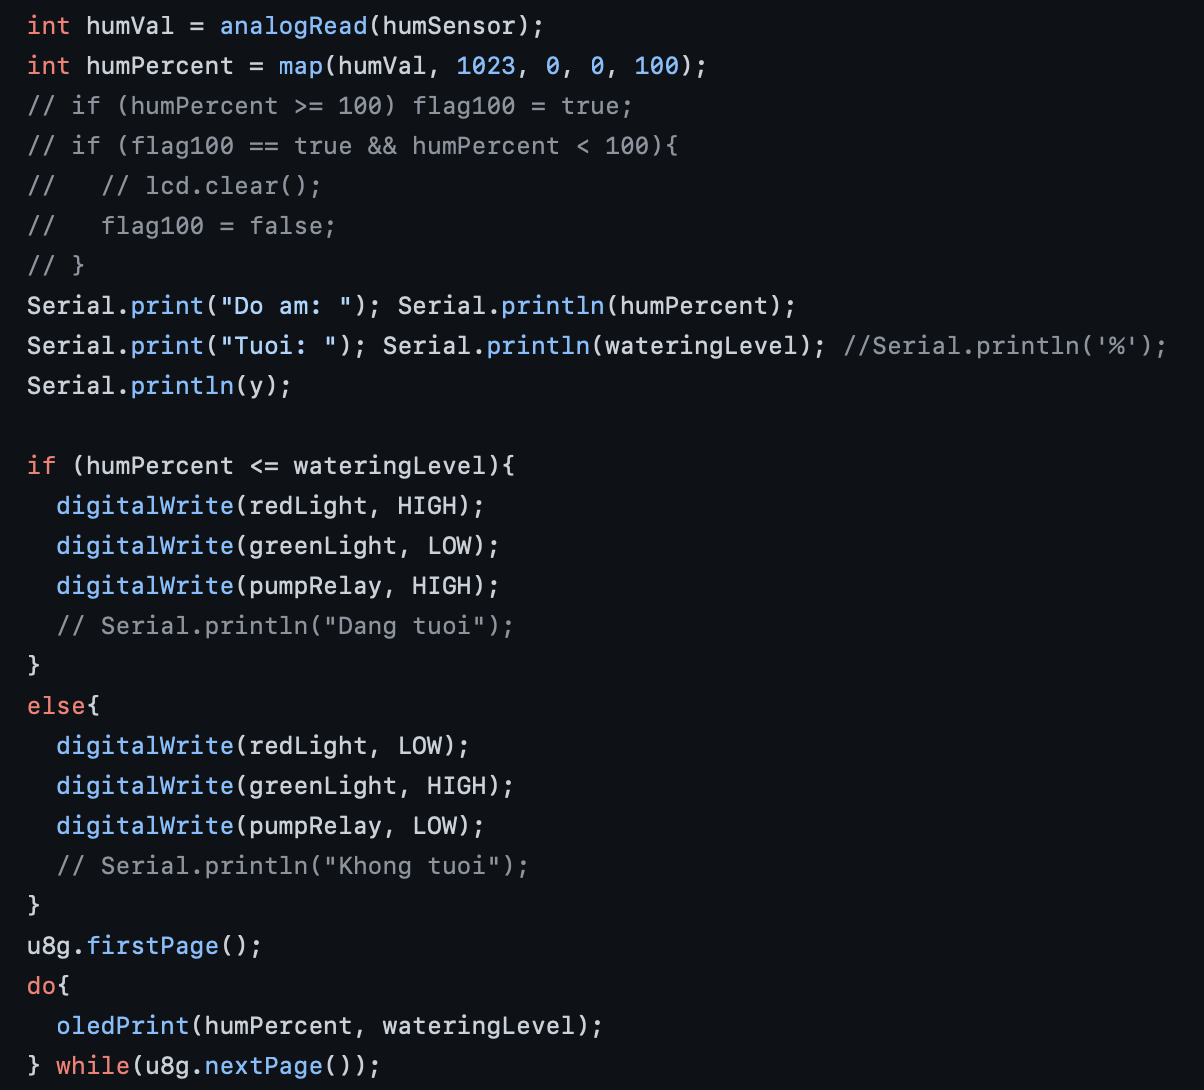
\includegraphics[width=14cm]{./images/main2.png}
        \caption{Second part of the main code}
        \label{fig:main2}
    \end{figure}
    
    We declare integer humVal and assign the reading from the humidity sensor to it. We then proceed to declare integer humPercent and map humVal to it on scale of 0 to 100. After that, we make an if-else statement which enables the red LED and the relay module and disable the green LED when humPercent is less than or equal to wateringLevel and vice-versa. We call the oledPrint(humPercent, wateringLevel) function to print the two integer variables on the display.
    
    \begin{figure}[H]
        \centering
        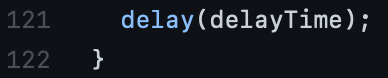
\includegraphics[width=14cm]{./images/main3.png}
        \caption{Final part of the main code}
        \label{fig:main3}
    \end{figure}
    
    This means that the loop runs once every 200 milliseconds.

    \section{Experiment}
    \begin{table}[H]
        \centering
        \begin{tabular}{|
        >{\columncolor[HTML]{FFFFFF}}c |l|l|l|
        >{\columncolor[HTML]{FFCCC9}}l |}
        \hline
        \cellcolor[HTML]{FFCC67}\textbf{Order} & \multicolumn{1}{c|}{\cellcolor[HTML]{FFCC67}\textbf{Description}}                                                          & \multicolumn{1}{c|}{\cellcolor[HTML]{FFCC67}\textbf{Detail}}                                                                                                    & \multicolumn{1}{c|}{\cellcolor[HTML]{FFCC67}\textbf{Result}} & \multicolumn{1}{c|}{\cellcolor[HTML]{FFCC67}\textbf{Issue}}                                                                                   \\ \hline
        \textbf{1}                             & \begin{tabular}[c]{@{}l@{}}2 seperate \\ power supplies\end{tabular}                                                       & \begin{tabular}[c]{@{}l@{}}5W power supply for \\ Arduino UNO \\ and components\\ \\ 1W power supply \\ for water pump\end{tabular}                             & \cellcolor[HTML]{67FD9A}Good                                 & \begin{tabular}[c]{@{}l@{}}Have to plug in \\ 2 power supplies\end{tabular}                                                                   \\ \hline
        \textbf{2}                             & \begin{tabular}[c]{@{}l@{}}5V - 0.7A \\ power supply\end{tabular}                                                          & \begin{tabular}[c]{@{}l@{}}5V - 0.7A power \\ supply for the \\ whole circuit\end{tabular}                                                                      & \cellcolor[HTML]{FFCCC9}Unstable                             & \begin{tabular}[c]{@{}l@{}}Not enough power \\ causing components \\ to turn off randomly\end{tabular}                                        \\ \hline
        \textbf{3}                             & \begin{tabular}[c]{@{}l@{}}12V - 0.45A \\ power supply\\ \\ Same voltage \\ for all components\end{tabular}                & \begin{tabular}[c]{@{}l@{}}12V - 0.45A power \\ supply for the \\ whole circuit\\ \\ 5V for all components\end{tabular}                                         & \cellcolor[HTML]{FFCCC9}Unstable                             & \begin{tabular}[c]{@{}l@{}}Overheating\\ \\ Not enough power \\ causing Arduino \\ UNO to reset \\ when the pump \\ is activated\end{tabular} \\ \hline
        \textbf{4}                             & \begin{tabular}[c]{@{}l@{}}12V - 0.45A \\ power supply\\ \\ Different voltages \\ for different \\ components\end{tabular} & \begin{tabular}[c]{@{}l@{}}12V - 0.45A power \\ supply for the \\ whole circuit\\ \\ 5V for Arduino UNO \\ and components\\ \\ 3.3V for water pump\end{tabular} & \cellcolor[HTML]{67FD9A}Good                                 & \cellcolor[HTML]{67FD9A}No issue                                                                                                              \\ \hline
        \end{tabular}
    \end{table}

    \section{Implementing}
        \subsection{List of electronic devices}
            \begin{table}[H]
                \centering
                \begin{tabular}{|c|l|c|}
\hline
\multicolumn{1}{|l|}{STT} & Linh kiện                             & \multicolumn{1}{l|}{Số lượng} \\ \hline
1                         & Full wave rectifier AC-DC 12VDC 450mA & 1                             \\ \hline
2                         & Voltage source T89                    & 1                             \\ \hline
3                         & Oled 0.91 Inch I2C                    & 1                             \\ \hline
4                         & 5V water pump                         & 1                             \\ \hline
5                         & Red led                               & 1                             \\ \hline
6                         & Green led                             & 1                             \\ \hline
7                         & Andruino UNO                          & 1                             \\ \hline
8                         & Relay Module (5V-10A)                 & 1                             \\ \hline
9                         & Siphon                                & 1                             \\ \hline
10                        & Joystick                              & 1                             \\ \hline
11                        & Breadbroad                            & 1                             \\ \hline
12                        & Wires                                 & 25                            \\ \hline
13                        & Humidity Sensor                       & 1                             \\ \hline
\end{tabular}
\end{table}
        \subsection{Process}
        \begin{itemize}
            \item We place all the electronic components on the plastic flat surface. 
            \item We add wire for all the components like the Design section. 
            \item We choose the wire with the dark color for the GND and the bright color for the VCC.
            \item We choose the thick wire for the voltage source.
            \item We connect 3v3 OUT of the voltage source to the relay module.
            \item We connect 5V OUT of the voltage source to the breadboard.
            \item We use red light when the water pump is running and green light when the water pump is not running.
            \begin{figure}[!h]
                           \centering
                            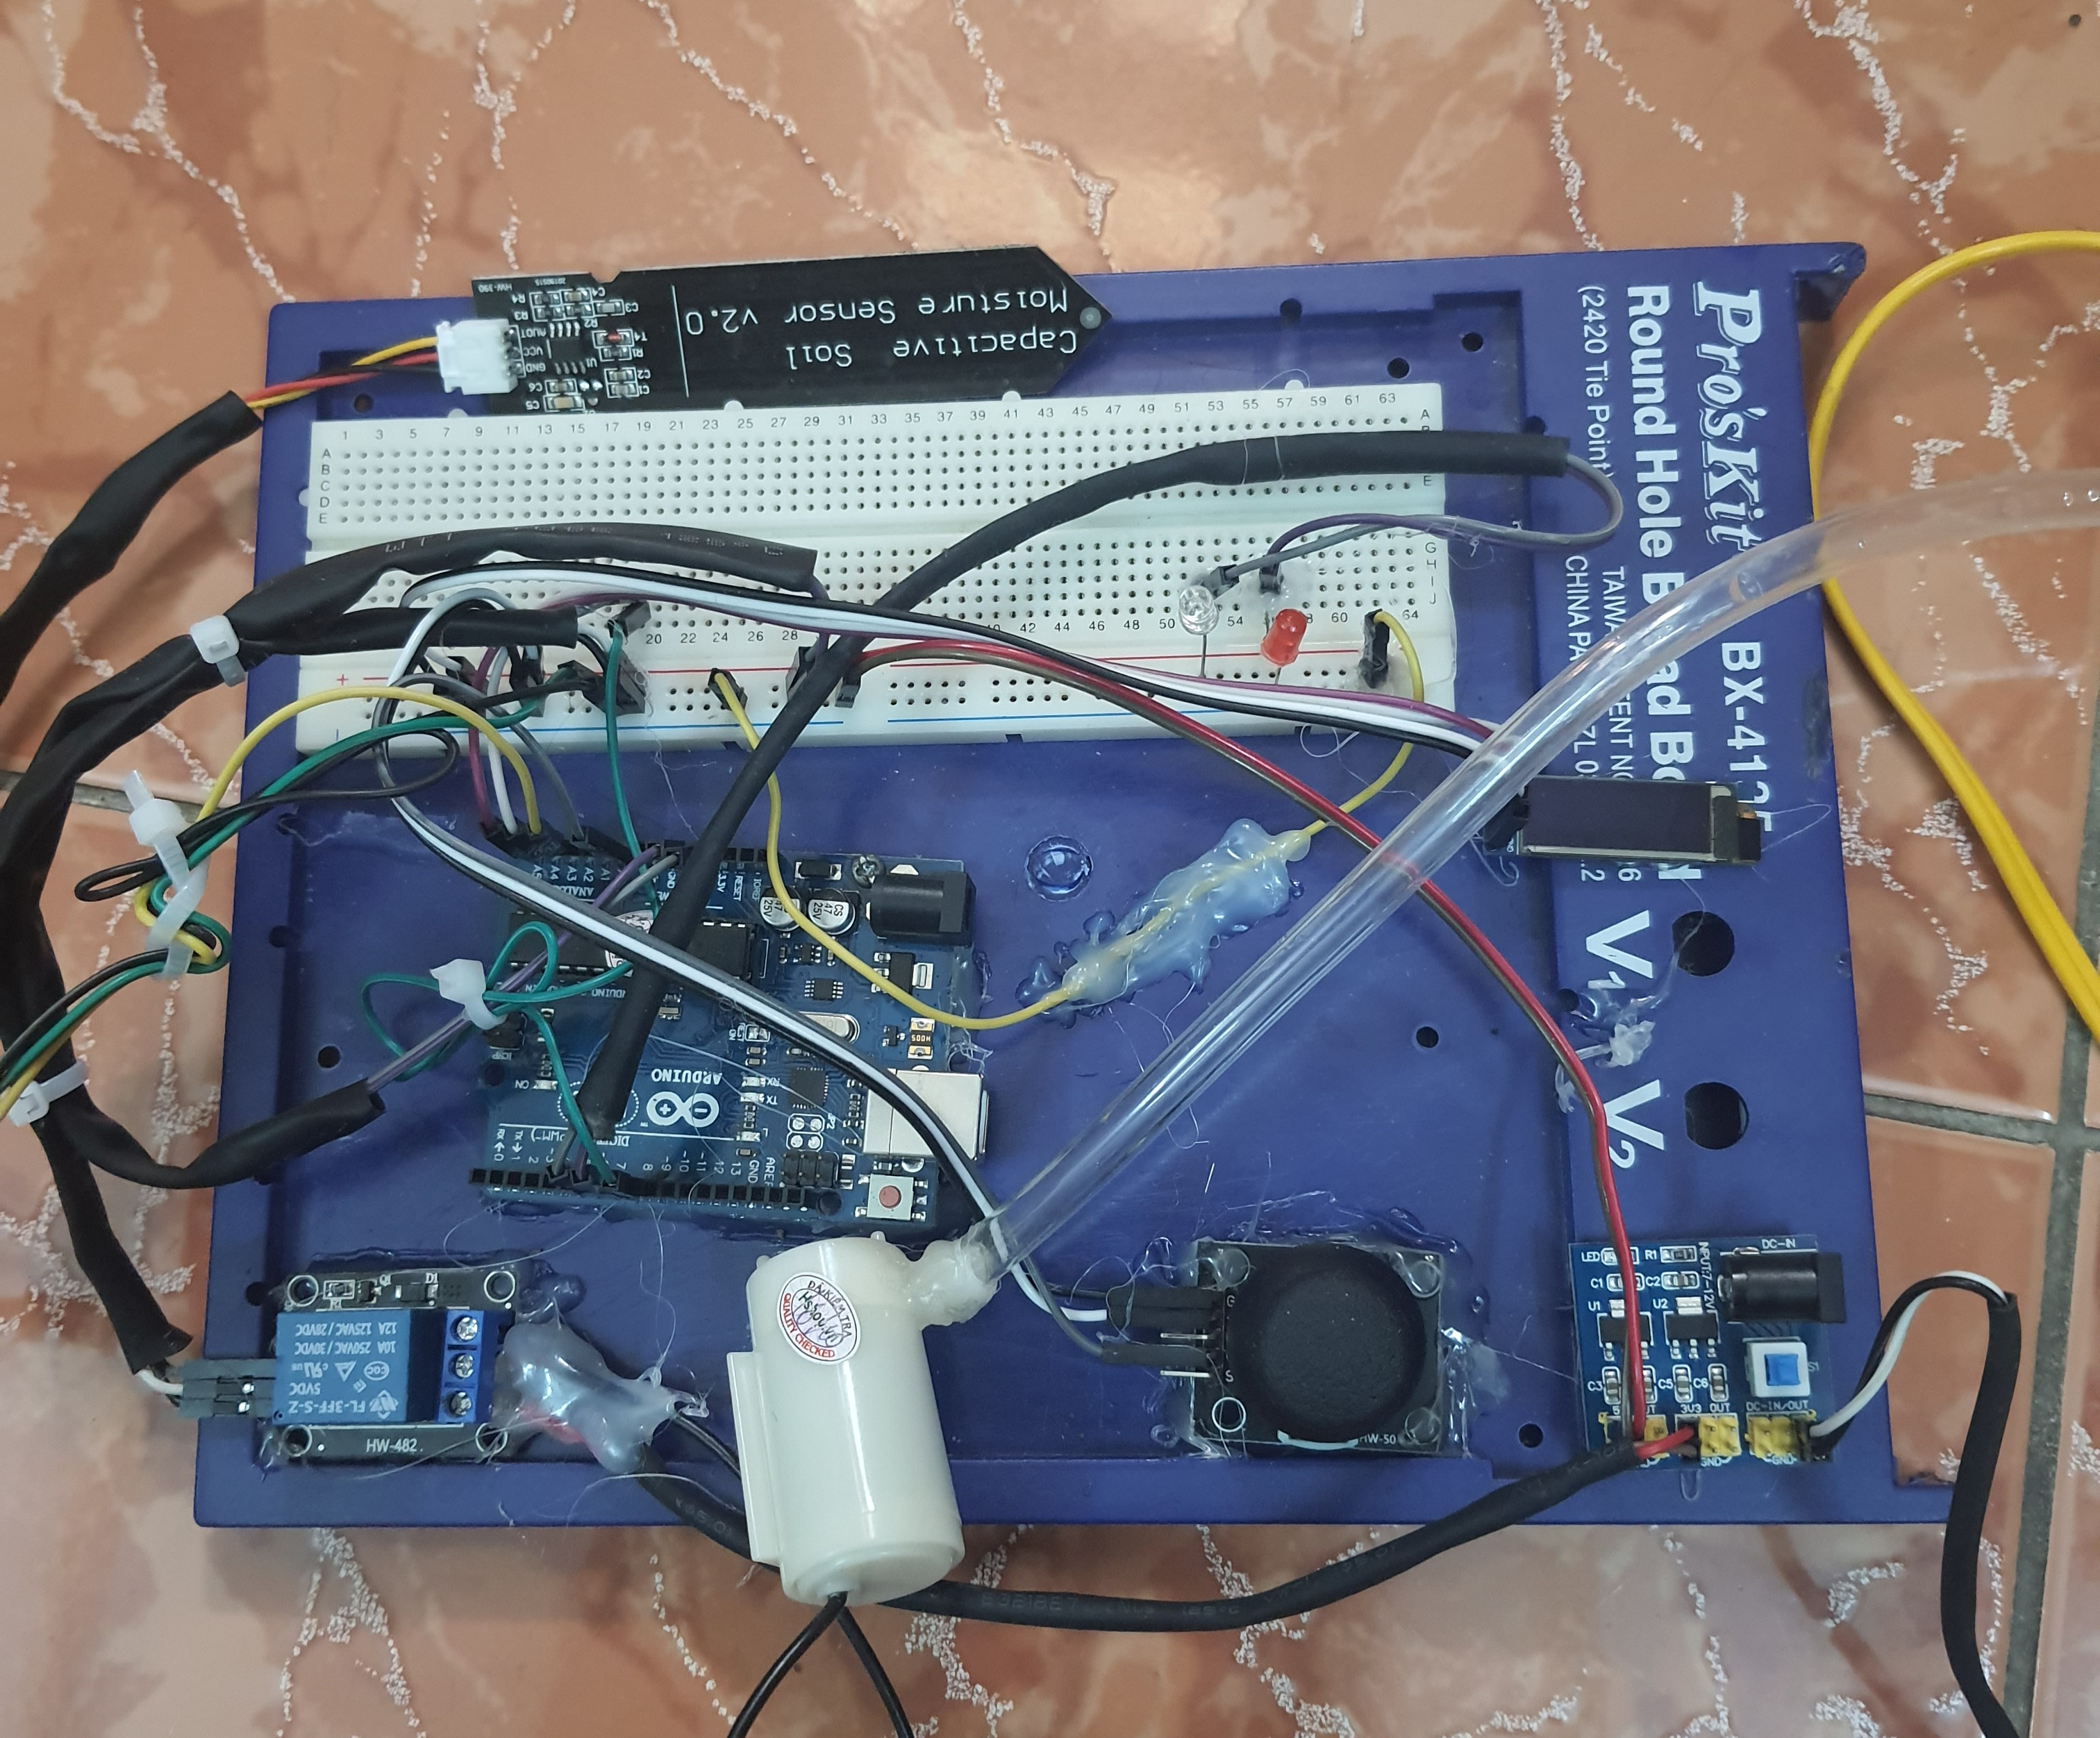
\includegraphics[width=14cm]{images/full_mach_dien.jpg}
                            \caption{The circuit}
                            \label{fig:schematic}
                    \end{figure}
        \end{itemize}
        \subsection{Advantages and disadvantages}
        \subsubsection{Advantages}
            \begin{itemize}
                \item Using breadboard instead of printing out the circuit let us can adjust the wire and do experiment easily.
                \item It's simple and easy to do.
                \item Good for learning purpose
            \end{itemize}
        \subsubsection{Disadvantages}
            \begin{itemize}
                \item A lot of wires so that the circuit looks tangled and not aesthetic.
                    \begin{figure}[!h]
                           \centering
                            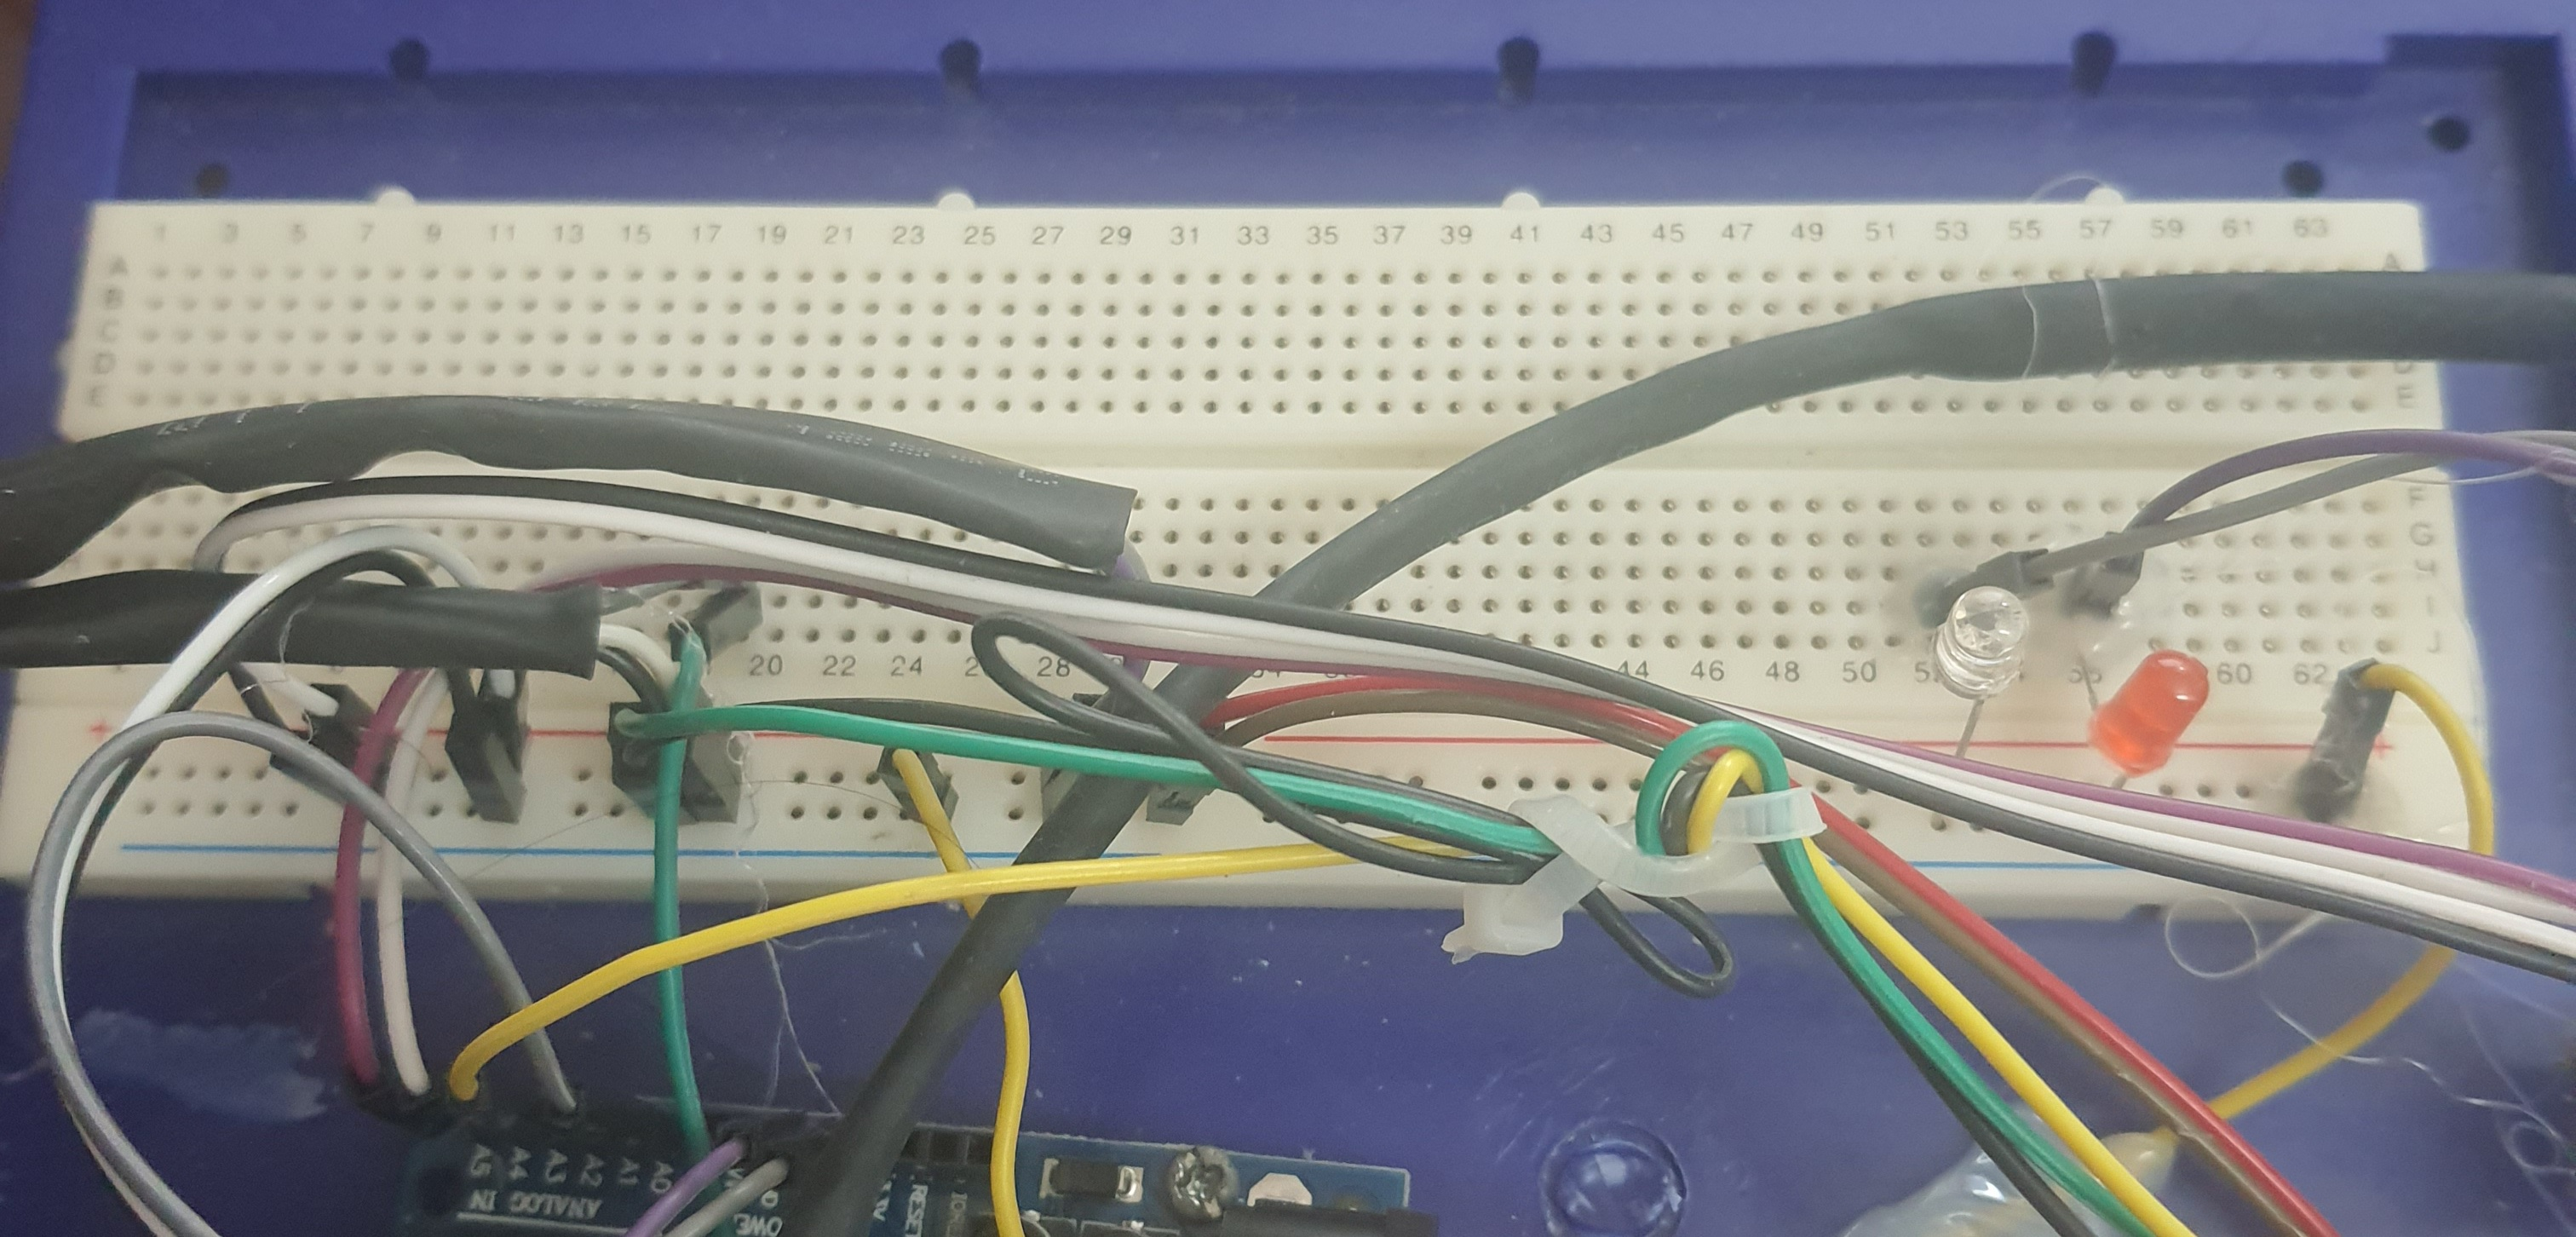
\includegraphics[width=14cm]{images/day_roi.jpg}
                            \caption{Tangled wires in the circuit}
                            \label{fig:schematic}
                    \end{figure}
                \item Easy to plug in the wrong wire, causing circuit damage.
                \item When we install the wire, the wire can break easily.
                    \begin{figure}[!h]
                           \centering
                            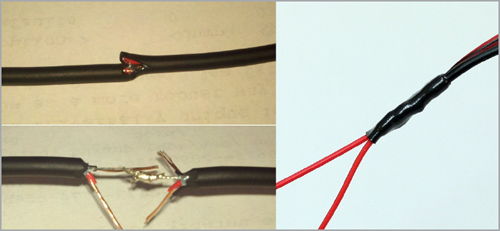
\includegraphics[width=14cm]{images/daydien.png}
                            \caption{Broken wire}
                            \label{fig:schematic}
                    \end{figure}
            \end{itemize}
    \section{Result}
        \subsection{Achievement}
            As we know, water is a very precious resource and must be used economically. Irrigation is a time consuming process and must be done on a timely basis. This moisturing-and-watering device can
            \begin{itemize}
                \item keep the plant always well-watered on a regular basic.
                \item save as much water as possible.
                \item require no human involvement (The circuit is based mainly on Arduino UNO and a soil moisture sensor).
            \end{itemize}     
         If the moisture is lower than the default moisturizing (30\% for example), the green led is on, the pump will water the plant. Otherwise, the red led is on (which means the plant's humidity is enough) \\  \\  
         You can checkout our result more clearly in the live-demo.
        \subsection{Deficiency}
            This plant moisturing-and-watering device can only be used for such small area
\end{document}